\documentclass[a4paper,12pt]{ctexart}

\usepackage{listings}
\usepackage{indentfirst}
\usepackage{xcolor}
\usepackage[colorlinks,linkcolor=black]{hyperref}
\usepackage{graphicx}
\usepackage{geometry}
\geometry{top=2.5cm,bottom=3.0cm,left=2.0cm,right=2.0cm}
\lstset{
	columns=fixed,
	numbers=left,
	breaklines=true,
	frame=shadowbox,
	commentstyle=\color{gray},
	rulesepcolor= \color{gray},
	numberstyle= \small,
	keywordstyle= \color{red},
	stringstyle=\rmfamily\slshape\color[RGB]{128,0,0},
	showstringspaces=false, 
	morekeywords={my,asm},
	showtabs=false,
	tabsize=4,
	title=\lstname,
	basicstyle=\ttfamily
}

\title{Android中的MVC}
\author{Will Also}
\date{2019}

\begin{document}
	\maketitle
	\tableofcontents
	\section{MVC}
	\subsection{MVC来源}
	MVC模式(Model–view–controller)是软件工程中的一种软件架构模式,把软件系统分为三个基本部分:模型(Model)、视图(View)和控制器(Controller)。
	\par MVC模式最早由Trygve Reenskaug在1978年提出,是施乐帕罗奥多研究中心(Xerox PARC)在20世纪80年代为程序语言Smalltalk发明的一种软件架构。MVC模式的目的是实现一种动态的程序设计,使后续对程序的修改和扩展简化,并且使程序某一部分的重复利用成为可能。除此之外,此模式透过对复杂度的简化,使程序结构更加直观。软件系统透过对自身基本部分分离的同时也赋予了各个基本部分应有的功能。
	\subsection{组件}
	\begin{itemize}
		\item 模型(Model) 用于封装与应用程序的业务逻辑相关的数据以及对数据的处理方法。
		 “Model”有对数据直接访问的权力,例如对数据库的访问。“Model”不依赖“View”和“Controller”,也就是说, Model 不关心它会被如何显示或是如何被操作。但是 Model 中数据的变化一般会通过一种刷新机制被公布(观察者模式)。
		 \item 视图(View)能够实现数据有目的的显示。在 View 中一般没有程序上的逻辑。为了实现 View 上的刷新功能,View 需要访问它监视的数据模型(Model),因此应该事先在被它监视的数据那里注册。
		 \item 控制器(Controller)起到不同层面间的组织作用,用于控制应用程序的流程。它处理事件并作出响应。“事件”包括用户的行为和数据 Model 上的改变。
	\end{itemize}

		
		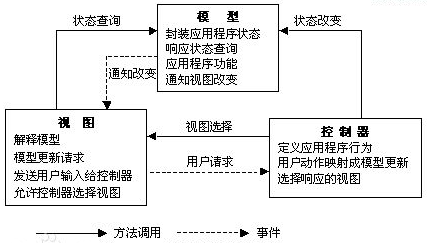
\includegraphics[]{image/1.png}
\end{document}
